% LaTeX version of report/report.odt.
%
% Build:  latexmk -pdf report.tex
%    or:  pdflatex report && pdflatex report
\documentclass[12pt,a4paper]{article}

\usepackage[T1]{fontenc}
\usepackage{lmodern}
\usepackage{microtype}
\usepackage[a4paper,margin=2.54cm,bottom=2cm]{geometry}
\usepackage{parskip}
\usepackage{amsmath}
\usepackage{graphicx}
\usepackage{booktabs}
\usepackage[font=small,labelsep=endash]{caption}
\usepackage{xcolor}
\usepackage{titlesec}
\usepackage{float} % [H]: figures stay exactly where they are in the text
\usepackage{setspace}
\usepackage[round]{natbib}
\usepackage{xurl}
\usepackage{hyperref}

\graphicspath{{figures/}}
\urlstyle{same}
\frenchspacing
\setcounter{secnumdepth}{0} % unnumbered headings, as in the original report

% Pages are broken by hand so that every page holds the same content as the
% original (see the "original p. N" comments). The looser line spacing makes
% pages fill about as much as the original's.
\raggedbottom
\setstretch{1.2}

% Colours taken from the original document
\definecolor{heading}{HTML}{0F4761}
\definecolor{link}{HTML}{467886}

\titleformat{\section}{\normalfont\LARGE\color{heading}}{}{0pt}{}
\titleformat{\subsection}{\normalfont\Large\color{heading}}{}{0pt}{}

% Lists without extra space between items, as in the original
\newcommand{\tightlist}{\setlength{\itemsep}{0pt}\setlength{\parskip}{0pt}}

\renewcommand{\contentsname}{Table of Contents}
\renewcommand{\refname}{List of References}
\renewcommand{\bibsection}{\section{\refname}} % also lists it in the TOC
\setlength{\bibhang}{0.5cm}

% Dotted leaders for top-level TOC entries too
\makeatletter
\renewcommand*{\l@section}{\@dottedtocline{1}{0em}{1.5em}}
\makeatother

\hypersetup{
  pdftitle={Investigation into repurposing the DART Network to study the
    Thermohaline Circulation},
  pdfauthor={Leon Huang},
  colorlinks=true,
  allcolors=black,
  urlcolor=link,
}

\begin{document}

% Title page (counted as page 1, like the original)
\thispagestyle{empty}
\vspace*{\stretch{2}}
\begin{center}
  {\huge Investigation into repurposing\\
    the DART Network to study the\\
    Thermohaline Circulation\par}
  \vspace{1.5em}
  Leon Huang (297 151 994)
\end{center}
\vspace*{\stretch{3}}
\clearpage

% --- original p. 2
\phantomsection
\addcontentsline{toc}{section}{\contentsname} % the original lists itself
{\setstretch{1.6}\tableofcontents}
\clearpage

% --- original p. 3

\section{Abstract}

Understanding the deep ocean is critical for studying a changing world;
however, deep ocean data remain spatially and historically limited. GeoNet's
DART Network is an early warning detection system near New Zealand. The bottom
pressure recorder has a temperature sensor placed inside the device, recording
internal temperature. The objective of this report is to investigate the DART
Network temperature data and determine if it can be used as a direct
measurement of water temperature. Anomalies and patterns in the temperature
data were investigated across different sensors and timescales, as well as
compared to reliable Argo sources. The result showed that there was
considerable noise, but also useful areas in the data. A sinusoidal pattern
was captured in the diurnal cycle, and a similar temperature range to Argo
data suggests that the DART Network is able to capture changes in temperature,
despite having an incorrect direct base temperature measurement. The data is
less reliable when used below an hourly timescale, as the software seems to
have some type of hourly process that consistently influences the temperature
data on the hourly scale.

\section{Acknowledgements}

I would like to acknowledge Melissa Bowen for supervising and providing the
initial idea for this research project.

\clearpage

% --- original p. 4
\section{Introduction}

The Thermohaline Circulation is how the ocean distributes heat, salt,
nutrients and marine life all around the world. Understanding the
Thermohaline Circulation is crucial for predicting climate patterns,
sustaining marine ecosystems, and monitoring global heat transport. Despite
its significance, data on deep ocean currents remains limited due to the vast
and deep nature of the ocean.

Advancements in technology have led to greater data available through the
Deep Argo Program, deep mooring techniques, and occasional ship casting and
survey data. However, coverage and historical data of the ocean floor remain
limited. An existing deep ocean monitoring system, the ``Deep-ocean
Assessment and Reporting of Tsunami'' (DART) Network, has shown some
potential in improving deep ocean visibility.

The DART Network is an early tsunami detection system in New Zealand; it
consists of a Bottom Pressure Recorder (BPR) on the ocean floor to measure
changes in water pressure. Within the BPR is a temperature sensor used to
monitor internal component temperatures. This research project investigates
the DART Network internal temperature sensor data and its viability to be
repurposed as a direct measurement of local deep water temperatures. If
possible, it will improve the historical temperature data available and
increase the data coverage along the ocean floor.

\section{Literature Review}

The Thermohaline Circulation, often referred to as the Global Conveyor Belt,
is a series of large, interconnected ocean currents that control the movement
of the world's ocean water. Warm surface waters are transported into deep
underwater currents along the ocean floor, some of these currents take
thousands of years to resurface. The Thermohaline Circulation spans across the
five oceans, redistributing heat, salt, nutrients, dissolved gases, and marine
life around the world \citep{pauthenet2019}.

\newpage % --- original p. 5

\subsection{Thermohaline Circulation Structure}

The circulation is mainly driven by the differences in water density, which is 
a function of the water's temperature (thermo) and salinity (haline). Water
density is highest towards polar regions and the bottom of the ocean, where
temperatures are typically low and salinity is high. This is not always the
case, the subtropics have the saltiest surface water, yet the polar water is
still denser. This is due to temperature having a stronger influence on
density compared to salinity \citep{zika2015}.

The structure of the Thermohaline Circulation can be understood through the
``push'' and ``pull'' theories of what drives the circulation, described by
\citet{lozier2010}. These theories are a way to categorise the driving forces
of the Thermohaline Circulation. The ``push'' theory suggests that the
circulation is pushed by deep water formation in the polar regions, as new
deep water is created, it pushes existing deep water through the deep
circulation currents. Deep water forms during sea ice creation, when water
freezes, only pure water is frozen out of the ocean. The salt content is left
behind, making the remaining local water saltier. Combined with the low
temperatures of the polar regions, the water becomes dense and sinks to the
bottom of the ocean.

When deep water forms in the North Atlantic, it is known as the North Atlantic
Deep Water (NADW), which sinks and travels south along the eastern coasts of
North America and South America, as shown in Figure~\ref{fig:thermohaline}.
Deep water often travels along the western side of ocean basins, which is the
eastern side of continents, due to the Coriolis force; scientists have
referred to these currents as the Deep Western Boundary Currents (DWBC). It
will continue along this DWBC until it reaches the Antarctic Circumpolar
Current (ACC). The Antarctic has a similar deep water formation during its own
sea ice creation, the deep water sinks, forming the Antarctic Bottom Water
(AABW), which also connects to the ACC.

As its name suggests, the ACC is a current that circumnavigates the Earth,
surrounding the Antarctic. It is a unique current in that it has both a
surface and a deep current that flow in the same direction. Due to the lack of
landmass, there are only two places where the ACC deviates, one is south of
Africa, and the other is along New Zealand. Bottom water leaves the lower limb
of the ACC in these locations and creates the DWBC along the African continent
and the Pacific Islands.

Along these two DWBCs, upwelling occurs, causing the deep water in the lower
limb to rise to the surface. The ``pull'' theory here suggests that part of
the \pagebreak % --- original p. 6
Thermohaline Circulation is driven by the pulling force from this upwelling.
There are many factors for upwelling, common ones are the wind-driven Ekman
transport, warmer latitude, and bathymetry.

After the deep water has upwelled, it now travels westward along the surface
currents, driven by the prevailing winds in the low latitudes. It will
continue until it reaches the Atlantic Ocean, at which point it will head
north to fill in the surface water that had been used in deep water formation
in the North Atlantic and continue the cycle.

\begin{figure}[H]
  \centering
  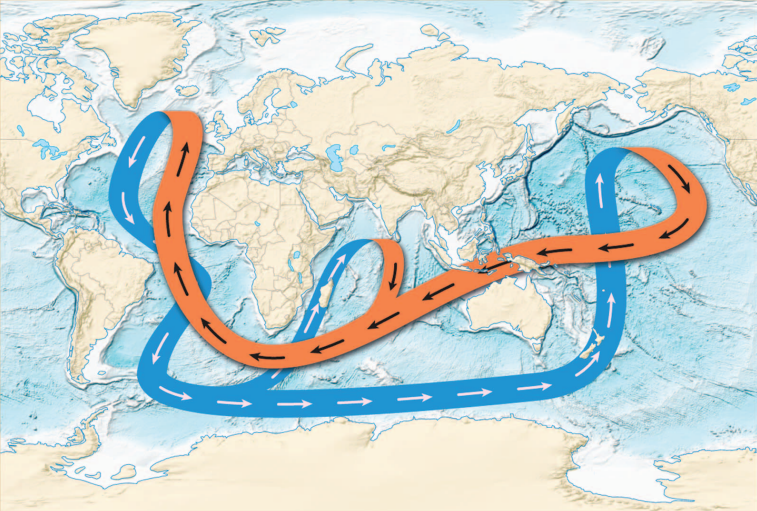
\includegraphics[width=\textwidth]{fig01_thermohaline_circulation}
  \caption{Diagram of Thermohaline Circulation. Orange represents warm
  surface water, while blue represents cold deep ocean water. Adapted from
  \citet{lozier2010}.}
  \label{fig:thermohaline}
\end{figure}

\subsection{Thermohaline Circulation around New Zealand}

Temperature and salinity are the main driving forces of the Thermohaline
Circulation. However, there are many other influences on the Thermohaline
Circulation, such as bathymetry, wind currents, climate modes, Coriolis force,
landmass, and numerous other global and local factors that affect specific
currents.

This research paper will focus on the Thermohaline Circulation around New
Zealand. New Zealand is situated near the strongest ocean current on Earth,
the ACC, and serves as the entry point to a DWBC. The ACC is a current that
circles the entire Antarctic continent. Unlike other currents, the ACC
encompasses the entire \pagebreak % --- original p. 7
vertical water profile, consisting of both a warmer surface current and a
cooler deep current that flows eastward \citep{niwa2008}.

On the east side of New Zealand sits another important current of the
Thermohaline Circulation, the DWBC. This current takes AABW from the lower
limb of the ACC around the east side of NZ and into the DWBC in the Pacific
Ocean, where it will resurface during upwelling \citep{niwa2008}.

When sea ice forms at the coast of Antarctica, only pure water is frozen while
the salt is rejected. This salt sinks into the deep ocean, increasing the
salinity and density of the deep waters. Katabatic winds from the Antarctic
Mountains come down and blow away newly formed sea ice, creating a continuous
cycle. This cycle of increasing salinity and decreasing temperature causes the
coastal water to sink due to density and travel northwards, providing the
dense water for the AABW \citep{silvano2023}.

The reason the ACC deviates around New Zealand is due to its southern
position but also the local bathymetry. This mainly refers to the wider
submerged continent New Zealand sits upon, Zealandia, distinguished by its
higher elevation above the surrounding oceanic crust \citep{mortimer2017}.

As a sunken continent, its elevation adds to the bathymetry, influencing
surrounding currents. South of New Zealand is the Macquarie Ridge, an
underwater mountain ridge that is an extension of the on-land Southern Alps.
The ridge sits along the ACC path, disrupting it and serving as the entry
point for AABW into the DWBC \citep{niwa2008}.

East of New Zealand is the Campbell Plateau and the Chatham Rise. These are
elevated pieces of underwater landmass extending eastward, outlining the
sunken Zealandia continent. After the AABW passes through the Macquarie
Ridge, the bathymetry deflects it northeast toward Campbell Plateau. Due to
the Campbell Plateau's elevated height, the AABW flows along the edge,
concentrating and intensifying the flow. This continues east along the Chatham
Rise, then turns north at its eastern edge into the Southwest Pacific,
providing the dense water in the DWBC \citep{carter1997}.

\newpage % --- original p. 8

\subsection{Data Availability}

These areas play a crucial role in the heat, salt, nutrient, and biological
processes surrounding New Zealand, and are worth researching and measuring.
Data on the Thermohaline Circulation is abundant for certain areas, while it
is extremely scarce in others. Technology such as satellites enables surface
current data to be abundant, but limited accessibility for the deep current
on the ocean floor \citep{carter1997}.

This research report is about data near New Zealand, so I will look at the
data available there. The most abundant data available, including around the
world, is sea surface temperature data from satellites. This type of data
collection is extremely efficient and has a large area of coverage. Radiation
emitted from an object depends on its temperature, so as long as the satellite
has a line of sight of the ocean, it is able to measure the ocean's
temperature. This type of data is collected and openly available from many
sources, such as \citet{niwa-satellite} or \citet{metservice}.

Another type of data available around New Zealand is from Argo. Argo floats
are devices at sea that float at various depths up to 2000 m below surface
level. These devices can record various information, including temperature and
salinity, at different layers before resurfacing and transmitting this
information to satellites. Argo data is part of the international Argo Program
that standardises and open-sources all the information collected around the
world. There are around 3,900 active Argo floats, and they are by far the
greatest source for below-surface data. New York Times science writer Justin
Gillis has described Argo as ``one of the scientific triumphs of the age''
\citep[as cited in][]{argoprogram}. But even Argo has its limitations, the
typical Argo float depth is limited to 2000m, and the position of a float is
dependent on the currents, so it cannot take continuous stationary samples.
There is a Deep Argo Program that can reach depths of 6000 m; however,
currently there are only about 200 active Deep Argo floats and even fewer near
New Zealand \citep{argoprogram}.

Mooring is another data collection technique that has been used around New
Zealand. This involves attaching measurement devices to a chain connected to
an anchor on one end and a buoy on the other. The device is left at a
stationary point at sea for a period of time, collecting a vertical
information profile. This has been done at the Macquarie Ridge, Campbell
Plateau, and Kermadec Trough near New Zealand. The limitations of mooring are
the small area of coverage, the fixed data period, and the extremely
\pagebreak % --- original p. 9 (starts at "many places" below)
high financial and labour cost. Additionally, many places are too dangerous to
use mooring techniques, such as the ACC due to the strong waves and stormy
weather \citep{niwa2008}.

\section{Objectives and Methods}

GeoNet is New Zealand's national geohazard monitoring organisation, one of
their monitoring systems is the DART network, an early tsunami detection
system. It does this through a device at the bottom of the ocean floor that
detects sudden changes in pressure, additionally it also has an internal
temperature recorder. My research supervisor, Melissa Bowen (2025), was first
to notice that the temperature data was mislabelled, it was listed as water
temperature when the sensor was placed inside the housing unit, and did not
have direct contact with water. The objective of my research project is to
investigate this internal temperature dataset and assess the viability of
repurposing it as a measurement of surrounding deep water temperatures.

\subsection{DART Network}

The DART Network uses devices on the sea floor to detect tsunami as a part of
an early warning system. The device on the sea floor is called the Bottom
Pressure Recorder (BPR), which uses the change in water pressure to detect
incoming tsunamis, typically intended for use after natural events such as
earthquakes. When a change is recorded, the BPR uses an acoustic signal to
communicate with a buoy, which in turn uses a faster electromagnetic signal to
communicate with satellites, which transfer all this data to an operating
centre \citep{geonet}.

The BPR has two modes. In its normal mode, it records data samples in
15 minute intervals; the samples are packaged and transmitted every 6 hours.
Once a significant change in water pressure is detected, it switches to event
mode. In event mode, data is sampled every 15 seconds and is immediately
transmitted; this continues for the next 3 hours before switching back to
normal mode. The BPR also records its internal temperature every 15 seconds,
but this data is not transmitted; it is stored locally and is only available
after maintenance, which occurs once every two years.

\newpage % --- original p. 10

\subsection{Objectives}

My research objective is to investigate the viability of using the DART
Network's BPR internal temperature data as a measurement for the temperature
of the surrounding deep water. The research objectives were:

\begin{enumerate}\tightlist
  \item Investigate the temperature pattern during event mode
  \item Investigate the temperature spike at the beginning of the data to see
  if a vertical temperature profile could be created
  \item Investigate the differences in temperature between sensors
  \item Investigate the data reliability by comparing it to Argo data
  \item Investigate any natural and human patterns in the data
\end{enumerate}

\subsection{Methods}

Most of the investigation was conducted using one sensor at one station for
the sake of time and efficiency. Since I am motivated to investigate the
dataset to study the Thermohaline Circulation, the station closest to it was
chosen. There are five stations close to New Zealand; however, all five of
these are north of the Chatham Rise and are not along the east edge where the
AABW travels. Station NZE was chosen because it is the easternmost of the five
and will most likely be the closest to the DWBC as it travels towards the
Pacific Ocean.

\begin{enumerate}\tightlist
  \item The data used in this investigation is from \citet{gns2020} as part of
  the New Zealand GeoNet program sponsored by the Natural Hazards Commission
  (NHC), Land Information New Zealand (LINZ), the National Emergency
  Management Agency (NEMA) and the Ministry of Business, Innovation and
  Employment (MBIE). I used the GeoNet API to access the data, while using the
  Python packages of pandas and matplotlib to graph and do correlation
  analysis on the three main datasets of temperature, pressure, and height.
  \item To investigate the possibility of creating a vertical temperature
  profile with the data during descent, I graphed the temperature and height
  at the start of the data, when the descent would have been recorded.
  \item To investigate the differences in data between sensors, I created a
  function to simultaneously graph all the available sensors within a station
  with each other.
  \item To investigate the reliability of the data, I will compare it to deep
  Argo data, a well-known, reliable source for deep ocean data
  \citep{argo2025}. To access this data, I will use the Python package
  argopy.
  \item To investigate patterns, I will analyse the data on time-scales with
  known natural patterns, such as diurnal, lunar, and seasonal timescales.
\end{enumerate}

\newpage % --- original p. 11

\section{Results and discussion}

Plotting temperature data during both normal and event mode reveals anomalies
that will be investigated. Figure~\ref{fig:nze40-temperature} shows normal and
event mode temperature data plotted together. There are two types of spikes I
was interested in, those associated with event mode, and the spike at the
start, possibly related to the deployment. Additionally, there is a spike in
normal mode that did not correlate with a similar event mode response, around
July 2021, which will also be investigated.

\begin{figure}[H]
  \centering
  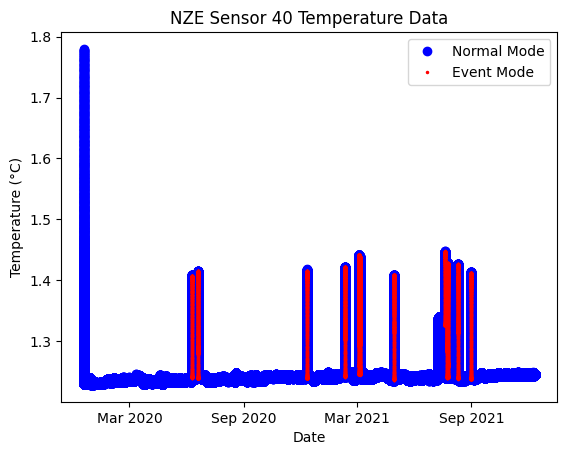
\includegraphics[width=0.68\textwidth]{fig02_nze40_temperature}
  \caption{Normal mode temperature data in blue and event mode temperature in
  red}
  \label{fig:nze40-temperature}
\end{figure}

When event mode is triggered, there is a consistent, sharp increase in
temperature. The temperature pattern at which the event mode ends is not as
consistent; however, it is always after the peak. This shows that the switch
to event mode does cause the device to produce more heat, affecting the data.
If this data is to be used to study the deep ocean, data relating to
event-mode should be cleaned. It should be noted that the temperature does
not immediately return to normal mode when event mode ends, as shown
in Figure~\ref{fig:event-mode}. This means that simply excluding data
associated with the exact time event mode starts and ends will still leave
traces in the data. It should be additionally noted that event modes have
been triggered without a sharp change in pressure; this could be done for
testing purposes, regardless the data is categorised under event mode.

\newpage % --- original p. 12

\begin{figure}[H]
  \centering
  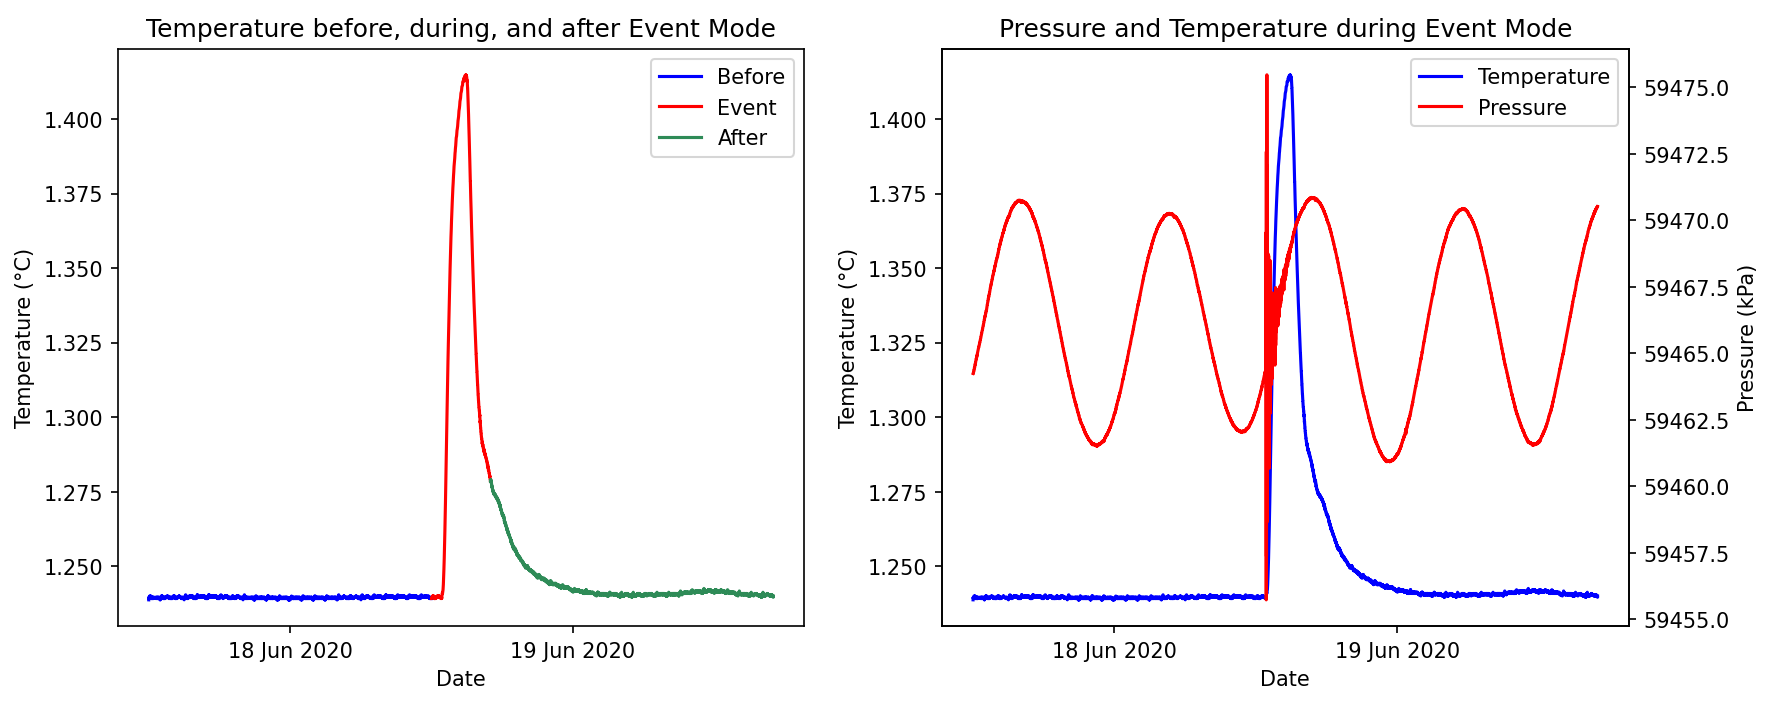
\includegraphics[width=0.96\textwidth]{fig03_event_mode}
  \caption{Left highlights the period before, during, and after the event
  mode. The right shows the corresponding changes in pressure during the
  period}
  \label{fig:event-mode}
\end{figure}

Investigating the temperature spike at the beginning of the data was to see if
the BPR had recorded temperature data during its descent. The hope was that if
it did, height data might have also been recorded; the combination of height
and temperature data would mean that a vertical temperature profile could be
formed.

Figure~\ref{fig:first-7-days} shows the first 7 days of temperature and
height data revealing a negligible difference in height throughout the 7
days. Though height peaked at the start, the range of height was less than
2m, nowhere near the amount needed for this degree of change in temperature.
This temperature spike is likely related to the testing or set-up process of
the device, rather than a temperature difference due to different layers of
the ocean.

\begin{figure}[H]
  \centering
  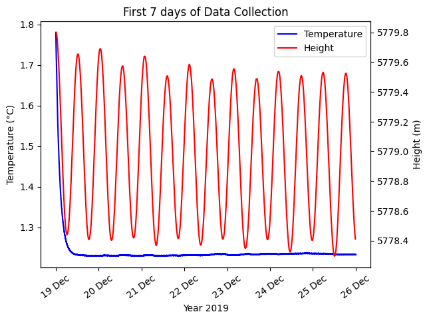
\includegraphics[width=0.68\textwidth]{fig04_first_7_days}
  \caption{The first 7 days of data, temperature on the left y-axis and
  height on the right y-axis}
  \label{fig:first-7-days}
\end{figure}

\newpage % --- original p. 13

On 9 July 2021, an unusual anomaly appeared in the data, the temperature
increased and remained between 1.30°C and 1.35°C for 13 days (see
Figure~\ref{fig:july-2021-anomaly}). After the 13 days, an event mode was
triggered without a change in pressure. After the event mode ended, it
returned to its regular temperature. This correlates with the increase in
temperature in Figure~\ref{fig:nze40-temperature} without an event mode
correlating with its duration. This is important to mention as it is another
type of anomaly that would need to be investigated if the dataset were to be
used. From the nature of the pattern, this could have been a software update
that triggered the temperature increase and ended with a test of the event
mode. Alternatively, something could have been wrong with the device, and a
manual trigger of the event mode fixed it.

\begin{figure}[H]
  \centering
  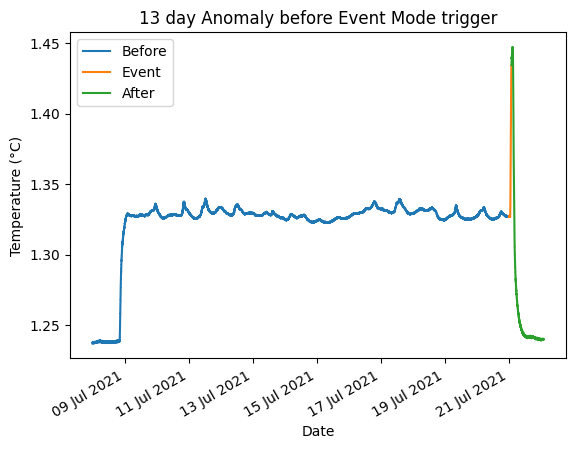
\includegraphics[width=0.58\textwidth]{fig05_july_2021_anomaly}
  \caption{Mysterious increase in temperature on 9 July 2021}
  \label{fig:july-2021-anomaly}
\end{figure}

A correlation graph between temperature and pressure yields interesting
results in Figure~\ref{fig:temp-pressure}. The most prominent feature on the
graph is the line that forms toward the top right. This line correlates to the
spike at the start of the data. The peak pressure along this line is also
similar to other points in the graph, which further supports that the initial
temperature spike is not due to temperature recording of different layers of
the ocean.

The next most interesting feature on the graph is the box-shaped pattern. The
top and bottom walls of the box are determined by pressure. The position of
these walls likely relates to the natural peaks and troughs of the tides. The
left and right walls of the box are determined by temperature. The left wall
is likely the normal state for the BPR, given how many points reside along it.
The right wall is likely the peak temperature during an event mode trigger;
the horizontal parabolic patterns with similar temperature maxima also support
this idea.

\newpage % --- original p. 14

Other noticeable patterns are the large number of points on the left wall that
are high and low in pressure. These points would have had a steady increase or
decrease in pressure such that there was no sudden change in pressure to
trigger event mode, allowing it to be recorded with low temperatures. The last
noticeable pattern is in the middle of the box. There is a large number of
points along a single temperature value between 1.3°C and 1.4°C. This likely
correlates to the previously mentioned anomaly on 9 July 2021, as it is the
only consistent data point at this temperature value.

\begin{figure}[H]
  \centering
  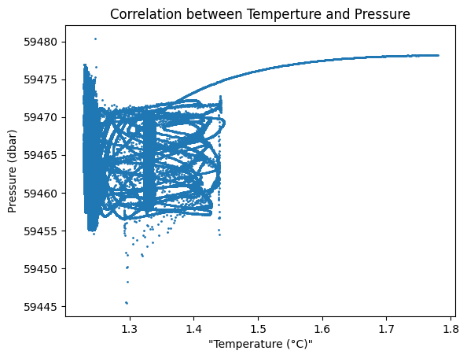
\includegraphics[width=0.63\textwidth]{fig06_temperature_pressure}
  \caption{Correlation graph between temperature and pressure}
  \label{fig:temp-pressure}
\end{figure}

Pressure is a function of depth in the ocean; the greater the depth, the
greater the pressure. As expected, examining the correlation between pressure
and height data reveals a strong correlation
(Figure~\ref{fig:height-pressure}), since the DART height is calculated from
the measured pressure.

\begin{figure}[H]
  \centering
  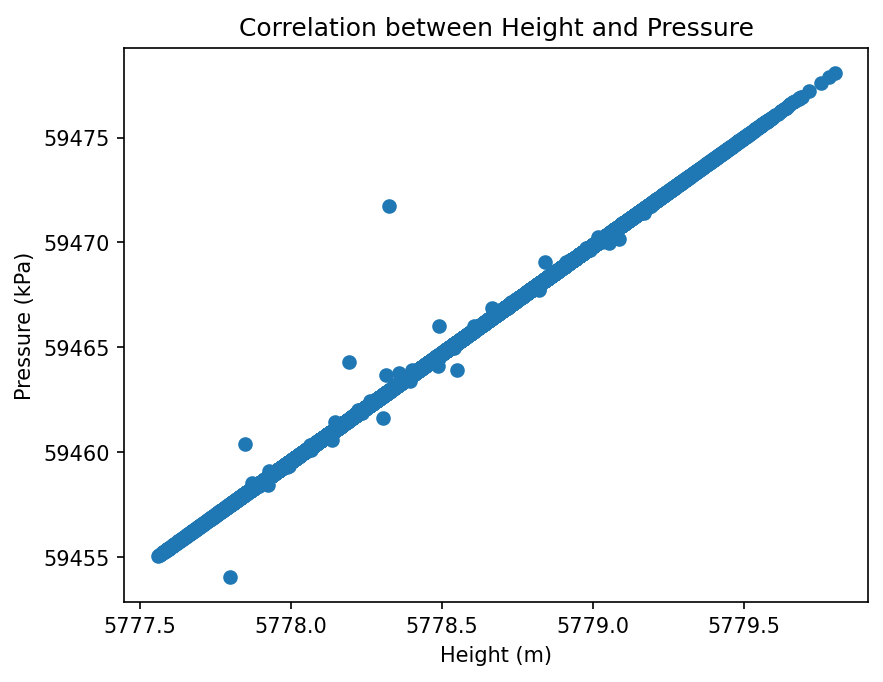
\includegraphics[width=0.58\textwidth]{fig07_height_pressure}
  \caption{Correlation graph between height and pressure}
  \label{fig:height-pressure}
\end{figure}

\newpage % --- original p. 15

\subsection{Sensor Comparison}

Having examined the data of station NZE's sensor 40, I next compared it with
other sensors. The NZE station has three sensors, 40, 41, and 42. Sensor
temperature data is stored locally on the BPR and is only available after
resurfacing during maintenance. As of this report, station NZE is active with
sensor 42. This means that only temperature data for sensors 40 and 41 is
available, while sensor 42 is not yet available. Comparing the temperature
data of these two sensors in Figure~\ref{fig:nze-sensors}, clear differences
are evident. The average of sensor 41 is 0.10°C higher than sensor 40.

\begin{figure}[H]
  \centering
  \begin{minipage}{0.5\textwidth}
    \centering
    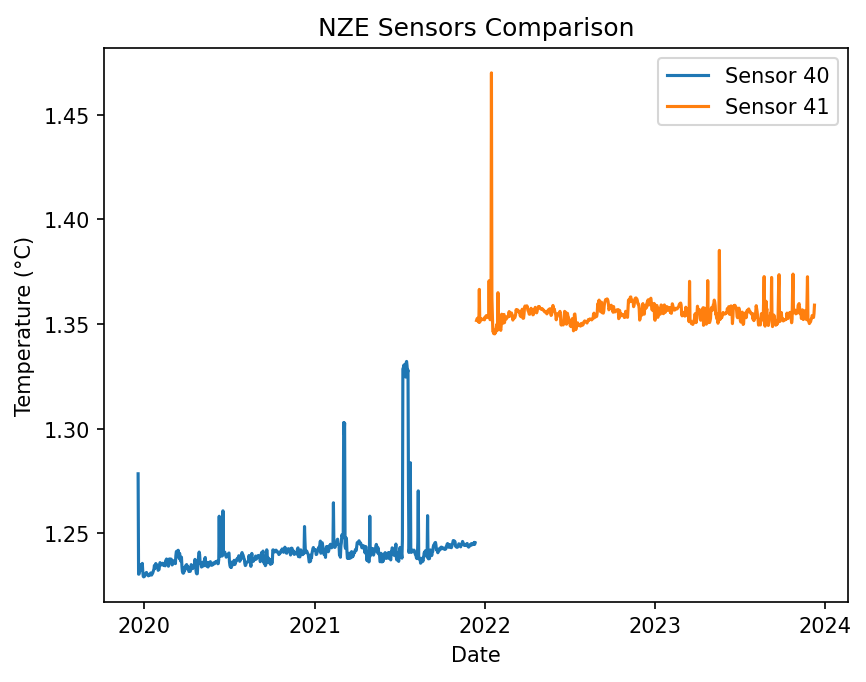
\includegraphics[width=\linewidth]{fig08_nze_sensors}
    \caption{Daily temperature data of station NZE sensors}
    \label{fig:nze-sensors}
  \end{minipage}\hfill
  \begin{minipage}{0.45\textwidth}
    \centering
    \begin{tabular}{lcc}
      \toprule
                & NZE 40           & NZE 41           \\
      \midrule
      Latitude  & $-36.0493^\circ$ & $-36.0399^\circ$ \\
      Longitude & $-177.708^\circ$ & $-177.697^\circ$ \\
      Elevation & $-5779$\,m       & $-5777$\,m       \\
      \bottomrule
    \end{tabular}
    \captionof{table}{Location of station NZE sensors}
    \label{tab:nze-locations}
  \end{minipage}
\end{figure}

Using the coordinates of each sensor provided by GeoNet, see
Table~\ref{tab:nze-locations}, a simple Pythagoras calculation can be done.

\[
  \sqrt{(111.32\,\text{km} \times 0.0094^\circ)^2
    + (111.32\,\text{km} \times \cos(36.04^\circ) \times 0.011^\circ)^2}
  \approx 1.44\,\text{km}
\]

Sensor 40 and sensor 41 were placed about 1.4 km apart with sensor 41 being
elevated 2 m higher. Considering the vastness of the ocean and the stability
of deep ocean temperatures, it is highly unlikely that a 1.4 km displacement
would cause a 0.10°C change in temperature. It is
more likely that some change in the equipment, be it the main components or
the temperature sensor itself.

\newpage % --- original p. 16

Figure~\ref{fig:station-sensors} examines the temperature data across all
sensors from every station, a shift in temperature occurs after every
maintenance. Some stations experienced similar increases in temperatures,
others experienced a decrease in temperatures, some looked to have no
significant change, while station NZJ nearly had a 2°C jump in temperature.
All the maintenance seems to have been done at three distinct points in time,
one near the start of 2022, one in the middle of 2022, and one in the middle
of 2023. All of which resulted in varying changes in temperature, and each
set of maintenance showed no consistent trend. It is difficult to say what the 
cause is just from the data alone. One possible explanation is that the 
temperature sensor was moved during maintenance, assuming there is no standard 
location for it. It is unlikely that equipment upgrades are the cause, as they 
would likely show some type of trend. If this data were to be used as accurate 
deep ocean temperature measures, considerable work would need to be done to 
recalibrate each sensor's data to an accurate norm.

\begin{figure}[H]
  \centering
  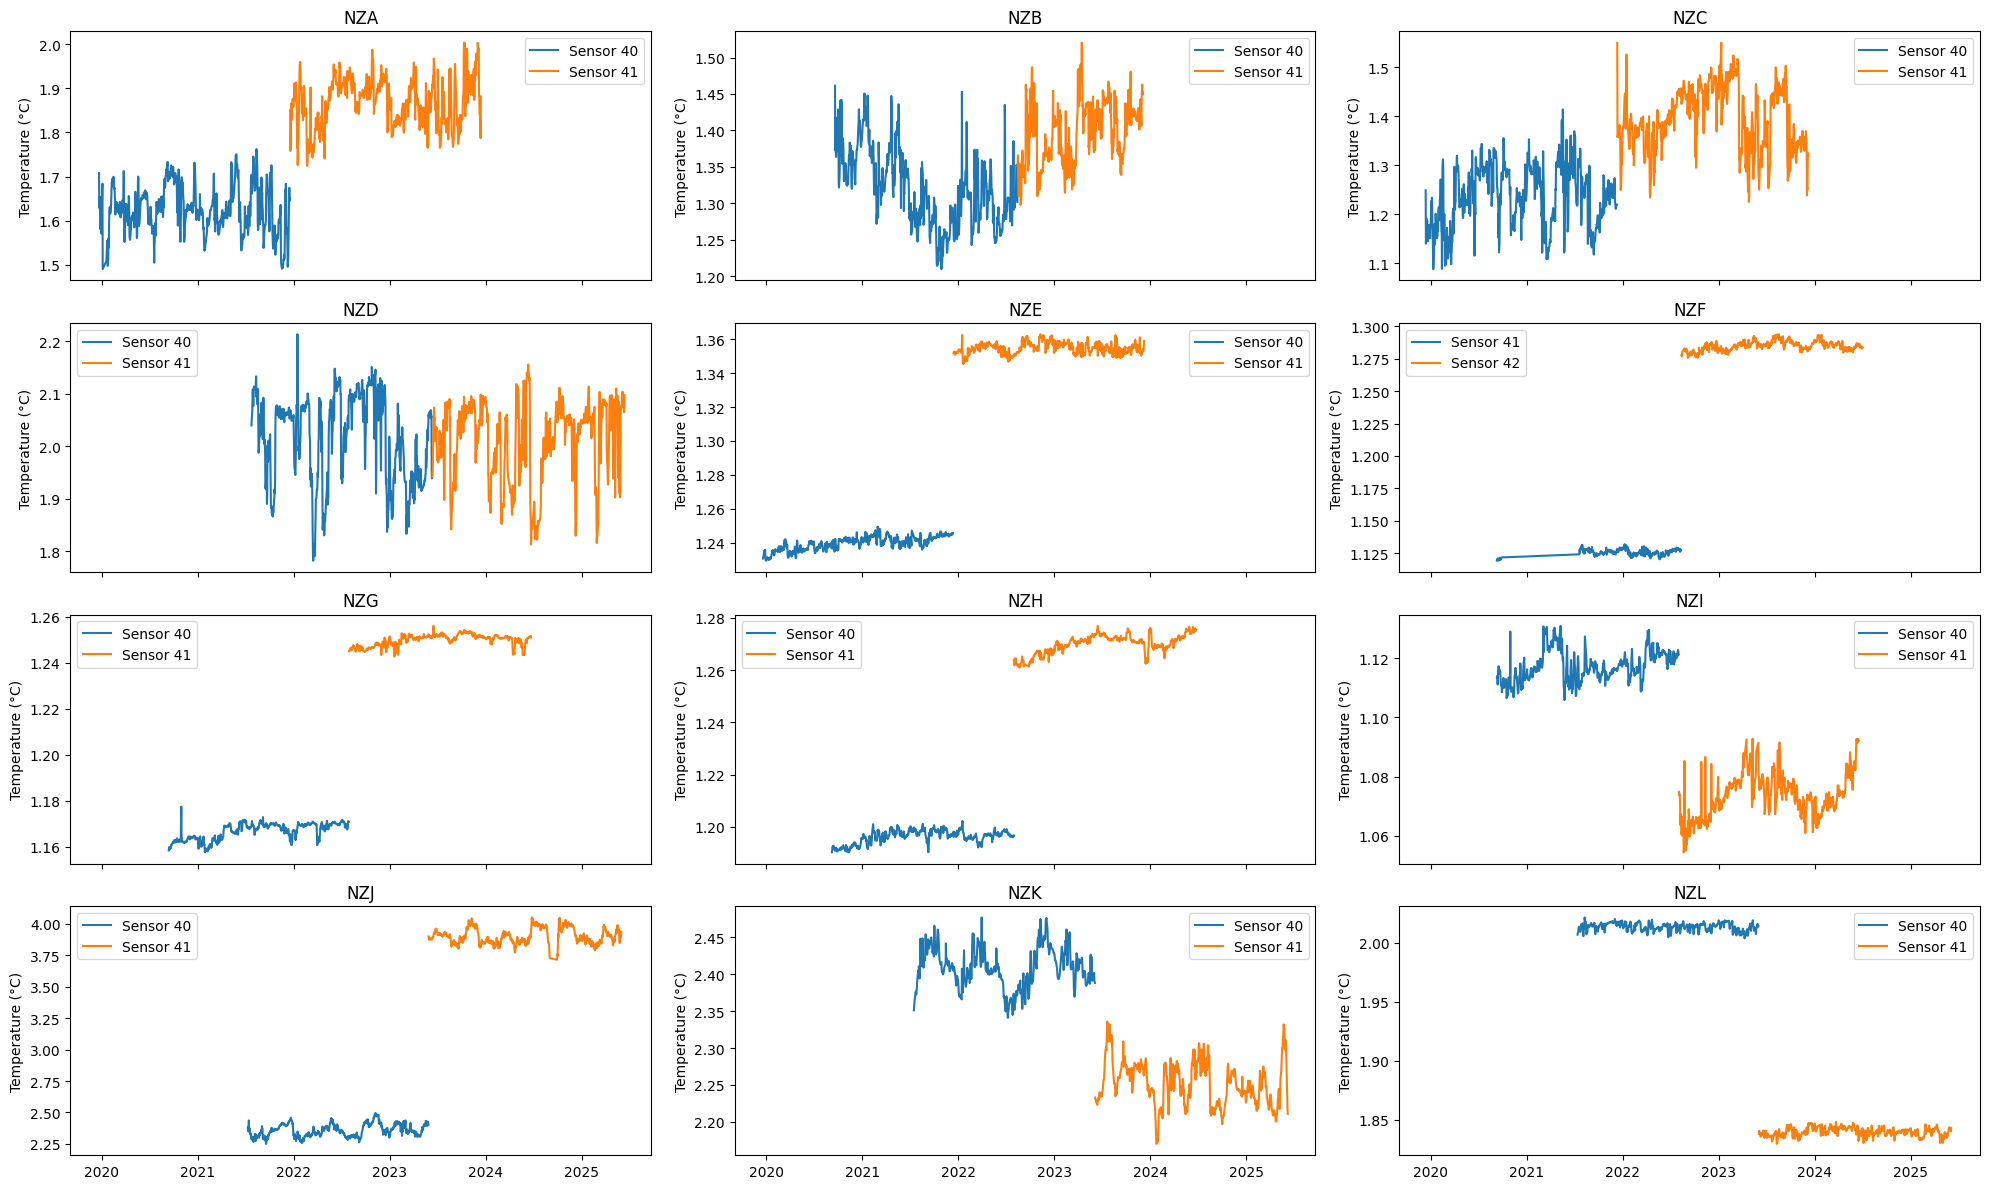
\includegraphics[width=\textwidth]{fig09_station_sensors}
  \caption{Comparison of sensors at each station, with outliers removed using
  the 1.5\,$\times$ interquartile range rule}
  \label{fig:station-sensors}
\end{figure}

\newpage % --- original p. 17

\subsection{Data reliability \& Argo Data}

Having examined the datasets, I next assessed their reliability in comparison
to other, more well-known data sources. From the deep Argo data, there are
some data points that are close to the location and depth of the station that
can be used. Comparing the available data points to the GeoNet data in
Figure~\ref{fig:argo-vs-dart} shows a clear disparity between the two. The
GeoNet data is consistently about 0.1°C higher than the Argo data. This
outcome is not surprising, considering that sensors have varying temperature
readings; it would not be reasonable to expect one to accurately record the
true temperature unless it were by chance.

\begin{figure}[H]
  \centering
  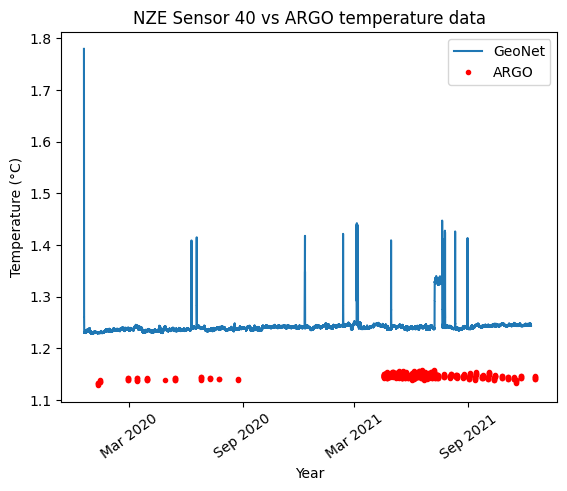
\includegraphics[width=0.55\textwidth]{fig10_argo_vs_dart}
  \caption{Argo temperature data in red and DART (GeoNet) temperature data in
  blue}
  \label{fig:argo-vs-dart}
\end{figure}

Though direct temperature measurements are not reliable, changes within the
data could be useful. Take the range shown in Figure~\ref{fig:argo-dart-range}
for example. Argo had a data range of 0.028°C, while NZE sensor 40 had a data
range of 0.025°C. The data ranges are quite similar; this could mean that
changes in the temperature data reflect changes in the surrounding
temperatures. Having a similar range is not enough to make it reliable for
representing temperature changes; it is uncertain whether this is caused by
changes in the surrounding water temperature or if the device simply produces
heat, causing a similar range.

\newpage % --- original p. 18

\begin{figure}[H]
  \centering
  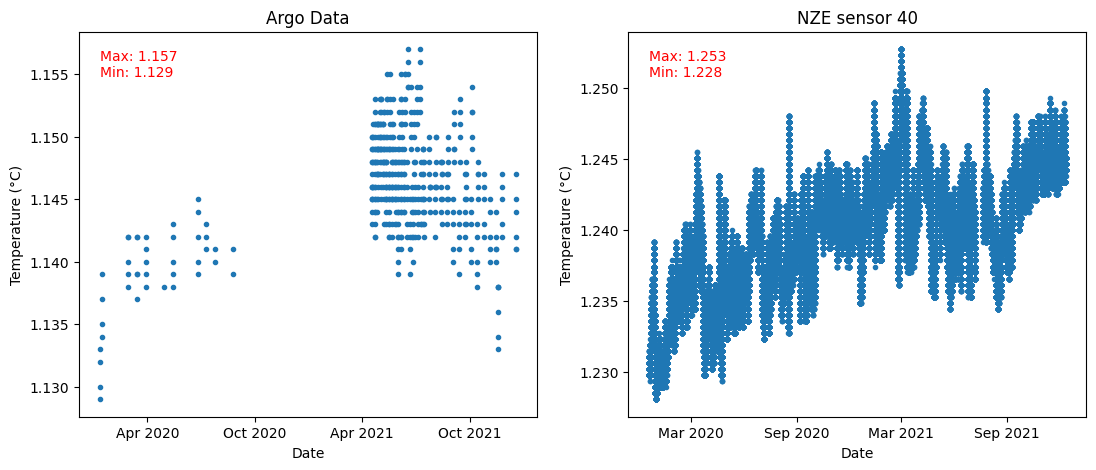
\includegraphics[width=0.88\textwidth]{fig11_argo_dart_range}
  \caption{Left is the Argo data, and right is the DART data with outliers
  removed. The maximum and minimum range is the top right of each graph}
  \label{fig:argo-dart-range}
\end{figure}

\subsection{Data Patterns}

Examining diurnal variation reveals clear natural and human patterns. Each
hour starts with a temperature spike and ends with a temperature drop. This
pattern is consistent every hour without fail, and is highly likely to be
related to the operation of the device. Without more details of the inner
workings of the device from GeoNet, it is difficult to determine if there are
any unaffected data points within each hour. As previously mentioned, the
DART Network transmits data every 6 hours in normal mode \citep{geonet}.
Interestingly, I could not find any 6-hour pattern with temperatures. Perhaps
the online information is incorrect, or the transmission of data produces
very little heat.

The natural pattern within a diurnal cycle is a sinusoidal pattern
(Figure~\ref{fig:diurnal}). This pattern is present each day, but the strength
and definition vary. The sinusoidal shape leads me to believe that this is
caused by the Earth's spin and the gravitational pull of the Moon and Sun,
similar to the tidal bulges. Further investigation with lunar and solar phase
data could yield very interesting results.

\begin{figure}[H]
  \centering
  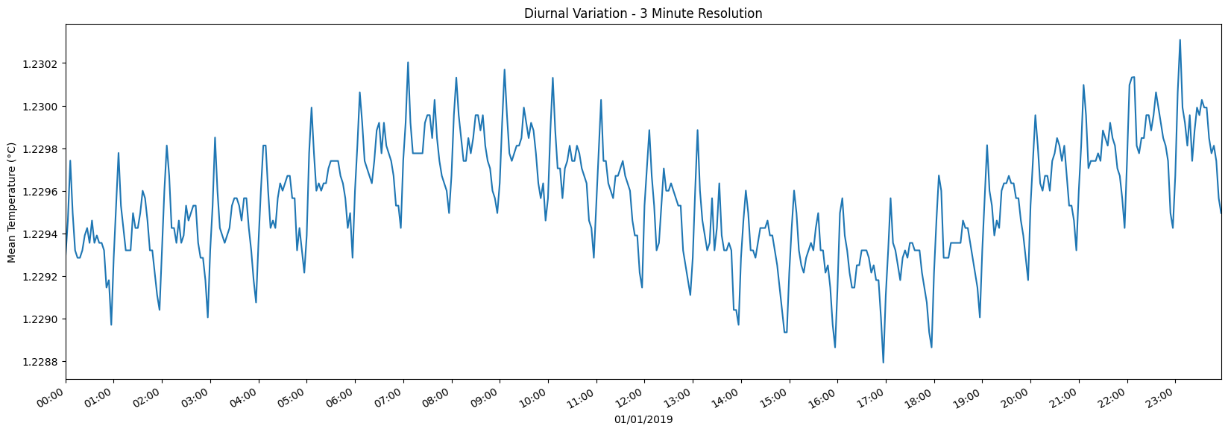
\includegraphics[width=\textwidth]{fig12_diurnal_cycle}
  \caption{The daily temperature on 1 January 2020 with points grouped into
  3-minute intervals}
  \label{fig:diurnal}
\end{figure}

\newpage % --- original p. 19

Examining the data on a yearly time-scale, I found no discernible patterns. I
specifically searched for yearly seasonal variations and monthly lunar
variations. Considering the gravitational pull theory suggested when
discussing the diurnal variation. The lack of patterns could suggest that the
moon and tilt of the Earth have little influence compared to the sun's 
gravitational pull on deep ocean temperatures.

\begin{figure}[H]
  \centering
  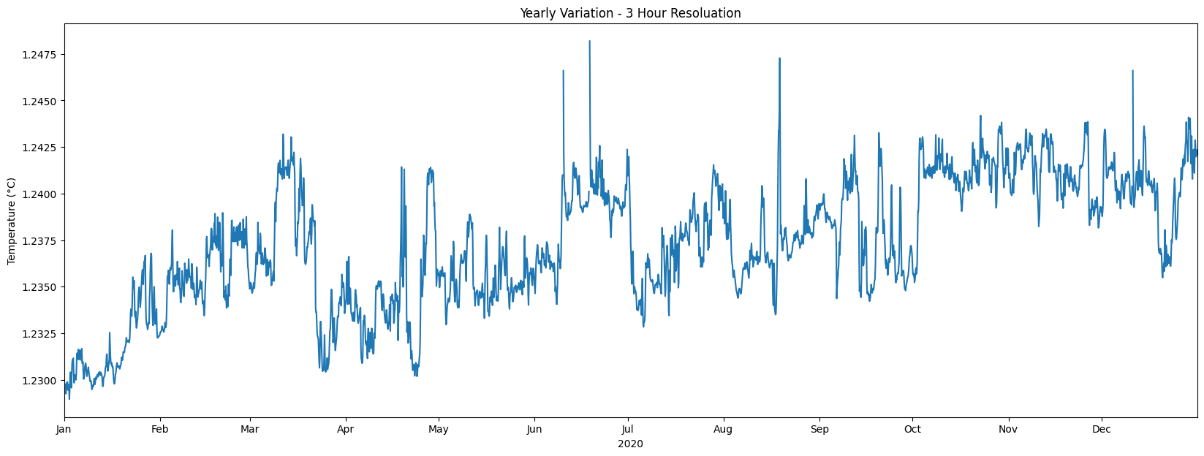
\includegraphics[width=\textwidth]{fig13_yearly_2020}
  \caption{2020 yearly temperature with points grouped into 3-hour intervals,
  after removing readings above 1.25°C}
  \label{fig:yearly}
\end{figure}

\section{Conclusion}

The DART Network temperature data from GeoNet contains a significant amount
of noise and requires extensive processing to be useful. Such as the
triggering of event mode, causing the temperature to rise. The temperature
spike at the beginning of the datasets is caused by the initiation after
deployment, and not temperature recording during the descent. Additionally,
there is an unexplained anomaly on station NZE sensor 40 starting on the 9 
July 2021. Using the data below an hourly resolution would need further work 
in understanding the inner software of the device.

The similar data range to the deep Argo data gives prospects for the dataset.
A similar data range could indicate that the dataset can be used to detect
temperature changes despite having different direct measurements; further
work is needed to understand the origin of the temperature in the device. The
sinusoidal pattern in the diurnal cycle is evidence that there are useful
natural patterns captured within the data. Further work with lunar and solar
cycle data could further confirm this, this work could also be helpful in
identifying if there are factors influencing the varying strength in the
sinusoidal pattern.

\clearpage

% --- original p. 20
\begin{thebibliography}{13}

\bibitem[Argo(2025)]{argo2025}
Argo. (2025). Argo float data and metadata from Global Data Assembly Centre
(Argo GDAC). SEANOE. \url{https://doi.org/10.17882/42182}

\bibitem[Argo Program(n.d.)]{argoprogram}
Argo Program. (n.d.). About. Scripps Institution of Oceanography, University
of California San Diego. Retrieved August 18, 2025, from
\url{https://argo.ucsd.edu/about/}

\bibitem[Carter \& McCave(1997)]{carter1997}
Carter, L., \& McCave, I. N. (1997). The sedimentary regime beneath the deep
western boundary current inflow to the Southwest Pacific Ocean.
\emph{Journal of Sedimentary Research, 67}(6), 1005--1017.
\url{https://doi.org/10.1306/d42686b2-2b26-11d7-8648000102c1865d}

\bibitem[GeoNet(n.d.)]{geonet}
GeoNet. (n.d.). DART (Deep-ocean Assessment and Reporting of Tsunami).
\url{https://www.geonet.org.nz/about/tsunami/dart}

\bibitem[GNS Science(2020)]{gns2020}
GNS Science. (2020). GeoNet Aotearoa New Zealand Deep-ocean Assessment and
Reporting of Tsunami (DART) dataset [Dataset].
\url{https://doi.org/10.21420/8TCZ-TV02}

\bibitem[Lozier(2010)]{lozier2010}
Lozier, M. S. (2010). Deconstructing the conveyor belt. \emph{Science, 328}(5985),
1507--1511. \url{https://doi.org/10.1126/science.1189250}

\bibitem[MetService(n.d.)]{metservice}
MetService. (n.d.). Sea surface temperature. Retrieved August 18, 2025, from
\url{https://www.metservice.com/maps-radar/marine/sea-surface-temperature}

\bibitem[Mortimer et~al.(2017)]{mortimer2017}
Mortimer, N., Campbell, H. J., Tulloch, A. J., King, P. R., Stagpoole,
V. M., Wood, R. A., Rattenbury, M. S., Sutherland, R., Adams, C. J., Collot,
J., \& Seton, M. (2017). Zealandia: Earth's hidden continent. \emph{GSA Today,
27}(3), 27--35. \url{https://doi.org/10.1130/GSATG321A.1}

\bibitem[NIWA(2008)]{niwa2008}
NIWA. (2008). Linking the world's oceans: the Antarctic Circumpolar Current.
\emph{Water \& Atmosphere, 16}(4), 24--25. Retrieved August 17, 2025, from
\url{https://niwa.co.nz/sites/default/files/import/attachments/oceans.pdf}

\bibitem[NIWA(n.d.)]{niwa-satellite}
NIWA. (n.d.). NOAA satellite data. Earth Sciences New Zealand. Retrieved
August 18, 2025, from \url{https://niwa.co.nz/atmosphere/noaa-satellite-data}

\bibitem[Pauthenet et~al.(2019)]{pauthenet2019}
Pauthenet, E., Roquet, F., Madec, G., Sallée, J.-B., \& Nerini, D. (2019).
The thermohaline modes of the global ocean. \emph{Journal of Physical
Oceanography, 49}(10), 2535--2552.
\url{https://doi.org/10.1175/JPO-D-19-0120.1}

\bibitem[Silvano et~al.(2023)]{silvano2023}
Silvano, A., Purkey, S., Gordon, A. L., Castagno, P., Stewart, A. L.,
Rintoul, S. R., Foppert, A., Gunn, K. L., Herraiz-Borreguero, L., Aoki, S.,
Nakayama, Y., Naveira Garabato, A. C., Spingys, C., Akhoudas, C. H., Sallée,
J.-B., de Lavergne, C., Abrahamsen, E. P., Meijers, A. J. S., Meredith, M.
P., \ldots{} Lee, W. S. (2023). Observing Antarctic Bottom Water in the
Southern Ocean. \emph{Frontiers in Marine Science, 10}, Article 1221701.
\url{https://doi.org/10.3389/fmars.2023.1221701}

\bibitem[Zika et~al.(2015)]{zika2015}
Zika, J. D., Skliris, N., Nurser, A. J. G., Josey, S. A., Mudryk, L.,
Laliberté, F., \& Marsh, R. (2015). Maintenance and broadening of the ocean's
salinity distribution by the water cycle. \emph{Journal of Climate, 28}(24),
9550--9560. \url{https://doi.org/10.1175/JCLI-D-15-0273.1}

% The original list also had these, but the text never cites them, so they
% are left out. Uncomment an entry and cite it to bring it back.
%
% \bibitem[Abraham et~al.(2013)]{abraham2013}
% Abraham, J. P., et al. (2013). A review of global ocean temperature
% observations: Implications for ocean heat content estimates and climate
% change. \emph{Reviews of Geophysics, 51}(3), 450--483.
% \url{https://doi.org/10.1002/rog.20022}
%
% \bibitem[Internet Geography(n.d.)]{internetgeography}
% Internet Geography. (n.d.). What is global atmospheric circulation?
% Retrieved August 16, 2025, from
% \url{https://www.internetgeography.net/topics/what-is-global-atmospheric-circulation/}
%
% \bibitem[National Emergency Management Agency(n.d.)]{nema}
% National Emergency Management Agency. (n.d.). How does the DART network
% work? [Infographic]. New Zealand Government. (This link no longer works.)
% \url{https://www.civildefence.govt.nz/assets/Uploads/publications/tsunami/DARTnetwork-infographic.pdf}
%
% With both NIWA (n.d.) entries in the list, label them (n.d.-a) and (n.d.-b).
% \bibitem[NIWA(n.d.)]{niwa-copyright}
% NIWA. (n.d.). Copyright and conditions of NIWA data access and use.
% Retrieved August 18, 2025, from
% \url{https://niwa.co.nz/climate-and-weather/copyright-and-conditions-niwa-data-access-and-use}
%
% \bibitem[Sathyanarayanan et~al.(2021)]{sathyanarayanan2021}
% Sathyanarayanan, A., Köhl, A., \& Stammer, D. (2021). Ocean salinity changes
% in the global ocean under global warming conditions. Part I: Mechanisms in
% a strong warming scenario. \emph{Journal of Climate, 34}(20), 8219--8236.
% \url{https://doi.org/10.1175/JCLI-D-20-0865.1}
%
% \bibitem[Webb(2021)]{webb2021}
% Webb, P. (2021). 8.1 Earth's heat budget. In \emph{Introduction to
% oceanography}. RWU Pressbooks.
% \url{https://rwu.pressbooks.pub/webboceanography/chapter/8-1-earths-heat-budget/}

\end{thebibliography}

\end{document}
